\documentclass{article}

% TODO: Make this different for two-sided printing than for two-up printing
% (two-up should have equal L/R margins)
\usepackage[paperwidth=5.5in, paperheight=8.5in, twoside, top=0.8in, bottom=0.8in, inner=0.6in, outer=1.0in]{geometry}

\usepackage{caption}
\usepackage{subcaption}
\usepackage{graphicx}

\begin{document}
\author{James Babcock (jimrandomh@gmail.com)}
\title{Petrov Day}

% Ideas to incorporate {{{
%  X Move the Malthus bit to after three candles are lit (establishing the pattern)
%  X Incorporate a tree of extinct human relatives, in the section about evolution
%    Mention collapsed civilizations: Easter Island, that island hypothesized as being Atlantis, Mayans, etc
%    Work in a mention of Moloch
%    Discuss the post-WW2 measures as a way of ending on a positive note: formation of the UN, twinning, reaties
%  - Mention abandonment of nuclear powered rockets
%    Mention environmental successes
% }}}

% Quotes to maybe use {{{
%
% Through the years her work continued to yield surprising insights, such as
% the unsettling discovery that chimpanzees engage in primitive and brutal
% warfare. In early 1974, a “four-year war” began at Gombe, the first record
% of long-term “warfare” in nonhuman primates. Members of the Kasakela group
% systematically annihilated members of the “Kahama” splinter group. --Jane Goodall

% Most species do their own evolving, making it up as they go along, which is
% the way Nature intended. -–Terry Pratchett

% Most gods throw dice, but Fate plays chess, and you don’t find out til too
% late that he’s been playing with two queens all along. -–Terry Pratchett

% Man still bears in his bodily frame the indelible stamp of his lowly origin. –Charles Darwin
% }}}


\newcommand{\divider}{ %{{{
	% From http://tex.stackexchange.com/questions/32711/totally-sweet-horizontal-rules-in-latex
	\nointerlineskip \vspace{\baselineskip}
	\hspace{\fill}\rule{0.5\linewidth}{.7pt}\hspace{\fill}
	\par\nointerlineskip \vspace{\baselineskip}
} %}}}
\newcommand{\stagedir} [1] { %{{{
	\begin{itshape}
	#1
	\end{itshape}
} %}}}
\newcommand{\blockquote} [2] { %{{{
	\begin{center}
		\parbox{3.5in}{
			``#1''
			\begin{flushright}
				--- #2
			\end{flushright}
		}
	\end{center}
} %}}}
\newcommand{\blockquoteUnattributed} [1] { %{{{
	\begin{center}
		\parbox{3.5in}{
			``#1''
		}
	\end{center}
} %}}}
\newcommand{\blockspacing} [1] { %{{{
	\begin{center}
		\parbox{3.5in}{
			#1
		}
	\end{center}
} %}}}
\newcommand{\blockquoteUnmarked} [2] { %{{{
	\begin{center}
		\parbox{3.5in}{
			#1
			\begin{flushright}
				--- #2
			\end{flushright}
		}
	\end{center}
} %}}}
\newcommand{\poem} [2] { %{{{
	\begin{center}
		\parbox{3.5in}{
			#1
			\begin{flushright}
				--- #2
			\end{flushright}
		}
	\end{center}
} %}}}
\newcommand{\page} [1] { %{{{
	\divider
	#1
	\divider
	\newpage
} %}}}
\newcommand{\pageNoBottomDiv} [1] { %{{{
	\divider
	#1
	\newpage
} %}}}
\newcommand{\sidePage} [1] { %{{{
	\vspace*{0.2in}
	#1
	\newpage
} %}}}
\newcommand{\candelabrum} [1] { %{{{
	\begin{center}
		\includegraphics[width=3in]{#1}
	\end{center}
} %}}}
\newcommand{\candlePassing} { %{{{
	\begin{center}
		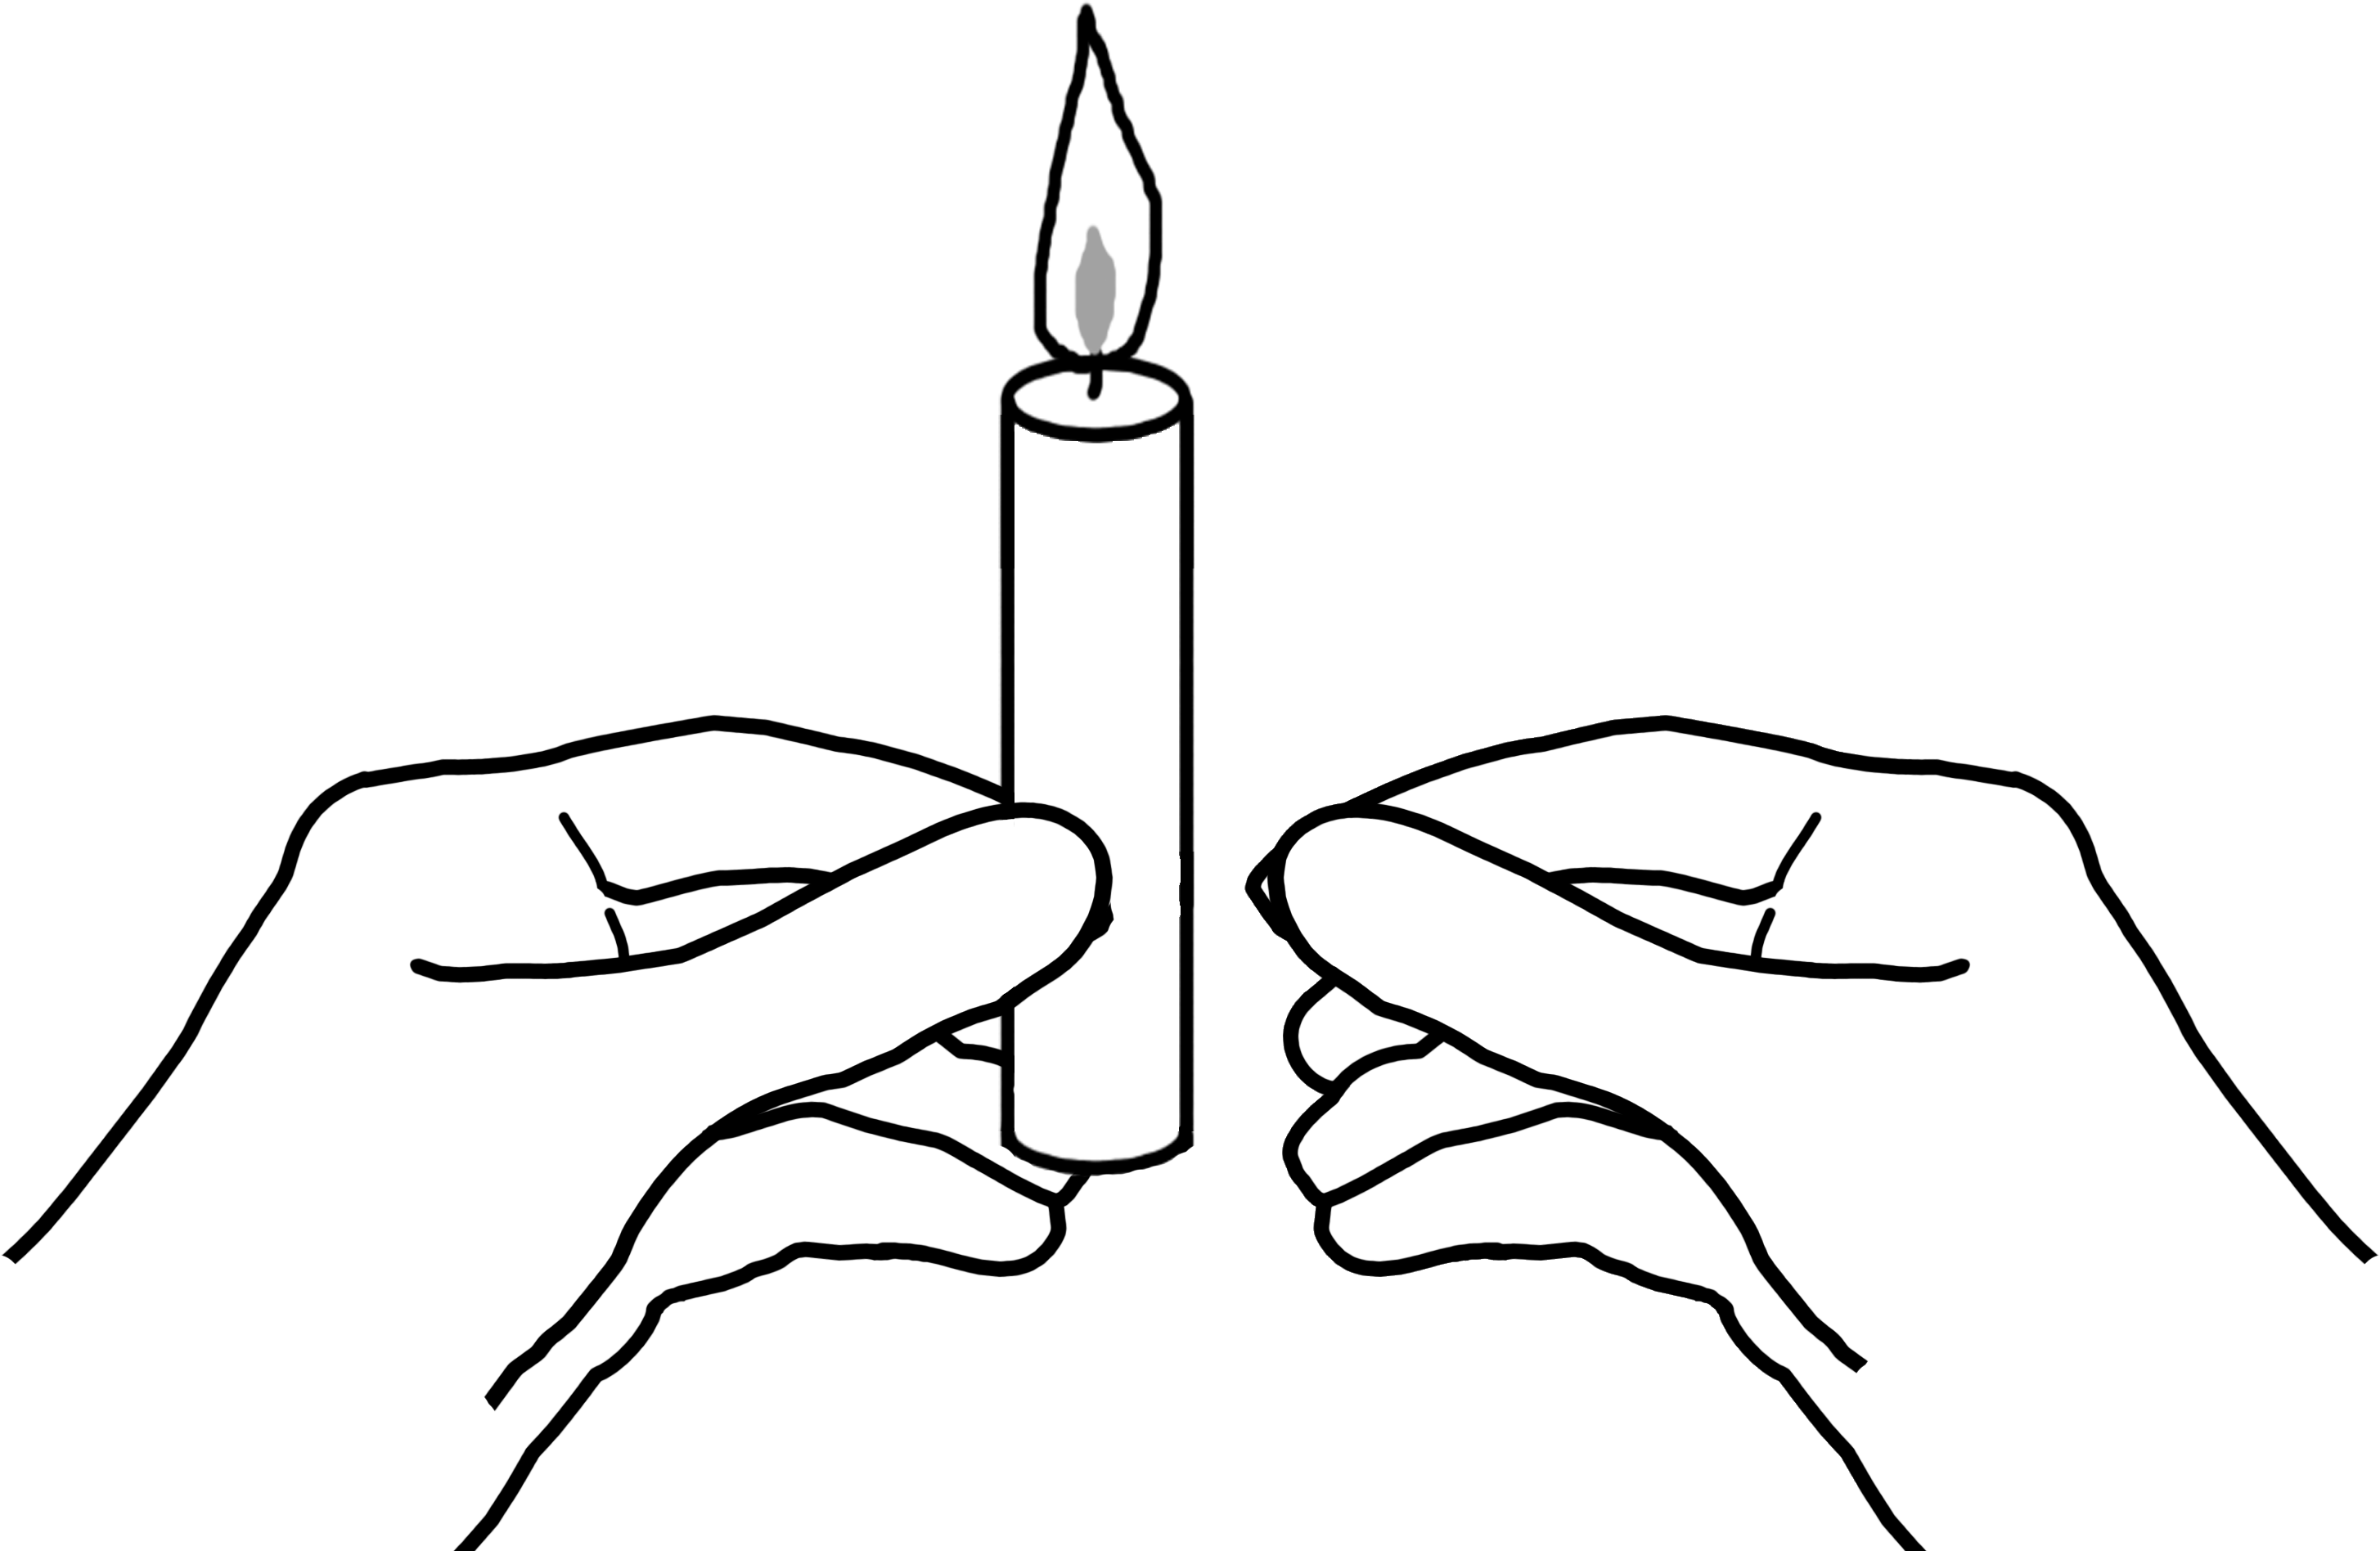
\includegraphics[width=2.5in]{images/candlepassing.png}
	\end{center}
} %}}}

% Don't indent paragraphs
\setlength{\parindent}{0cm}

\setlength{\parskip}{\baselineskip}

%%%%%%%%%%%%%%%%%%%%%%%%%%%%%%%%%%%%%%%%%%%%%%%%%%%%%%%%%%%%%%%%%%%%%%

% Front Matter
% Title page {{{
\pagenumbering{gobble}
\sidePage{

\begin{flushright}
\parbox{3in}{
	\begin{center}
		\Huge{Petrov Day}\newline
		\large{September 26}\newline
		\large{By James Babcock}\newline
	\end{center}
}
\end{flushright}

} % }}}
% What-is-this page 1 {{{
\pagenumbering{arabic}
\page{

Petrov Day is a yearly event on September 26 commemorating the anniversary of
the Petrov incident, where a false alarm in the Soviet early warning system
nearly set off a nuclear war. The purpose of the ritual is to make catastrophic
and existential risk emotionally salient, by putting it into historical context
and providing positive and negative examples of how it has been handled. This
is not for the faint of heart and not for the uninitiated; it is aimed at those
who already know what catastrophic and existential risk is, have some
background knowledge of what those risks are, and believe (at least on an
abstract level) that preventing those risks from coming to pass is important.

\divider

You will need:

\begin{itemize} \itemsep0pt \parskip0pt \parsep0pt
	\item A printout of this booklet for each person
	\item A table with enough chairs to seat everyone
	\item A candle holder
	\item 8 candles and a lighter
	\item A fire extinguisher close enough to retrieve if needed
	\item A deck of small index cards or a pad of post-it notes, and some pens
\end{itemize}

} % }}}
% What-is-this page 2 {{{
\page{

By James Babcock with content contributions by Ben Landau-Taylor, Adia Porter,
and Daniel Speyer, and quotations from many sources. Thanks to Eliezer Yudkowsky
for introducing the idea of commemorating Petrov Day, and to all the testers,
event organizers, and others who've made this possible.

} % }}}

% Introduction Section
% Intro page {{{
\page{

%\stagedir{Content warning: Engineered to evoke strong feelings of existential terror.}

\stagedir{Stage directions are written in italics, like this. All other text is
to be read aloud. Whenever there is a horizontal line, it becomes the next
person's turn to speak, going clockwise. When reading quotes, you don't need to
read the name and date at the end.}

This day, September 26, is Petrov Day. In 1983, the story of humanity nearly
ended. We're gathered here to remember that moment, and others like it. But to
really feel the magnitude of those events, we need to visit them in their
proper context. Let us begin the story of human history, starting from the
beginning.

\divider

\blockquote{In the beginning, the universe was created. This has made a lot of
people very angry, and been widely regarded as a bad move.}{Douglas Adams}

\divider

Let's fast forward over the thirteen billion year long prequel. Our story
begins in the age of myth, of fossils and legends. It starts with the invention
of fire.

} %}}}
% Prometheus quote: Light candle 1 {{{
\page{
\blockquote{I've hunted down and stolen, inside the hollow of a fennel's stalk,
the seed of fire, a gift that has proven itself to be the teacher of every craft
and the greatest resource for humans.  Such is the crime I have committed and
this is the penalty I am to suffer: nailed and chained on this rock beneath the
open sky.}{Prometheus Bound}

\candelabrum{images/candelabrum1.png}

\stagedir{Light the left-most candle, to represent the invention of fire. Point
out the location of the nearest fire extinguisher, then dim or turn off all
other lights in the room.}

} %}}}

% Prehistory

% About Fire {{{
\page {

Depending which archaeologists you ask, fire was first used by either Homo
Erectus or Homo Ergaster, some time between 400 thousand and 1.7 million years
ago. Cooking is believed to have enabled larger, more energy-intensive brains,
allowing the evolution of increased intelligence, and language.

\divider

\blockquote{Most species do their own evolving, making it up as they go along,
which is the way Nature intended. And this is all very natural and organic and
in tune with mysterious cycles of the cosmos, which believes that there's
nothing like millions of years of really frustrating trial and error to give a
species moral fiber and, in some cases, backbone.}{Terry Pratchett}

} %}}}
% Family tree {{{
\sidePage {

\newcommand{\skull} [2] { %{{{
	\parbox{1.3in}{
		\begin{center}
			\includegraphics[width=1.2in]{#1}
			#2
		\end{center}
	}
} %}}}

\skull{images/H_ergaster.png}{Homo Ergaster}
\skull{images/H_erectus.png}{Homo Erectus}
\skull{images/H_florensiensis.png}{Homo Florensiensis}
\skull{images/H_habilis.png}{Homo Habilis}
\skull{images/H_heidelbergensis.png}{Homo Heidelbergensis}
\skull{images/H_neanderthalis.png}{Homo Neanderthalis}
\skull{images/H_rudolfensis.png}{Homo Rudolfensis}


} %}}}
% CUT: Fire and speech {{{
%\page {
%
%Estimates place the invention of fire somewhere from 400,000 to 1.7 million
%years ago, while anatomically modern humans did not appear until 200,000 years
%ago.
%
%Fire is not, by itself, of particularly great importance. It grants protection
%from the cold of winter, and access to foods that would otherwise be inedible;
%but if it had stopped there, then the story of genus homo would have been
%unremarkable. But fire enabled, and favored, creatures with larger brains, and
%some time after that - we don't know when - our ancestors began to speak.
%
%} % }}}


% The invention of language: Candle 2 {{{
\pageNoBottomDiv{
%\blockquote{It's perfectly obvious that there is some genetic factor that
%distinguishes humans from other animals and that it is language-specific. The
%theory of that genetic component, whatever it turns out to be, is what is
%called universal grammar.}{Noam Chomsky}
% Source: http://www.slate.com/articles/health_and_science/new_scientist/2012/03/noam_chomsky_on_linguistics_and_climate_change_.html

\blockquote{It certainly is not a true instinct, for every language has to be learnt. It
differs, however, widely from all ordinary arts, for man has an instinctive
tendency to speak, as we see in the babble of our young children; whilst no
child has an instinctive tendency to brew, bake, or write.}{Charles Darwin,
Descent of Man (1871)}

} %}}}
% Language: Candle 2 {{{
\sidePage {

\stagedir{Take the first candle, which represents the invention of fire. Use it
to light the second candle, which represents the evolution of language.}

\candlePassing

\stagedir{Pass the candle once all the way around the circle. When you hold the
candle, it is your turn to speak. What is your name, and when (what year) is
your earliest memory?

\candelabrum{images/candelabrum2.png}

When everyone has spoken, put the candle back in the candelabrum.}

\divider

}
% }}}


% Agriculture: Candle 3 {{{
\page{

Language is the first key to technology; with it, early humans could accumulate
knowledge, not just in genes, but also in sayings and traditions.

They gave names to people around them. They gave names to species of animals
and plants. They gave names to actions and to places and to strategies. They
called some of these good, and called some of them bad. They learned to share
their knowledge, and they learned to deceive each other. They built families
and communities.

They began the long, slow process of taming the wilderness. Their tribes grew
to cities. What became of them?

\stagedir{Take the second candle, which represents language. Use it to light
the third candle, which represents agriculture.}

\candelabrum{images/candelabrum3.png}

} %}}}
% Uplift {{{
\sidePage {

\stagedir{If you or someone else at the table knows the tune to this song, then
sing; if not, read normally.}

\begin{center}
	\parbox{2in}{
		\begin{large}Uplift\end{large}\newline
		By Andrew Eigel
	}
\end{center}

\blockspacing{
	Hands chip the flint, light the fire, skin the kill\newline
	Feet move the tribe track the herd with a will\newline
	Mankind struggles in the cellar of history\newline
	Time to settle down, time to grow, time to breed\newline
	\newline
	Plow tills the soil, plants the seed, pray for rain\newline
	Scythe reaps the wheat, to the mill, to grind the grain\newline
	Towns and cities spread to empire overnight\newline
	Hands keep building as we chant the ancient rite}

\stagedir{Stop here. Go to the next page without reading or singing the rest of the song.}

\blockspacing{
	Coal heats the steam, push the piston, turns the wheel\newline
	Cogs spin the wool, drives the horses made of steel\newline
	Lightning harnessed does our will and lights the dark\newline
	Keep rising higher, set our goal, hit the mark.\newline
	\newline
	\-\hspace{0.5in}Crawl out of the mud,\newline
	\-\hspace{0.5in}Ongoing but slow,\newline
	\-\hspace{0.5in}For the path that is easy\newline
	\-\hspace{0.5in}Ain't the one that lets us grow!\newline
	\newline
	Light to push the sails, read the data, cities glow\newline
	Hands type the keys, click the mouse, out we go!\newline
	Our voices carry round the world and into space\newline
	Send us out to colonize another place¸\newline
	\newline
	Hands make the tools, build the fire, plant the grain.\newline
	Feet track the herd, build a world, begin again.}


}
% }}}


% The Malthusian Trap {{{
\pageNoBottomDiv {
\blockquote{The power of population is so superior to the power of the earth to
produce subsistence for man, that premature death must in some shape or other
visit the human race. The vices of mankind are active and able ministers of
depopulation.  They are the precursors in the great army of destruction, and
often finish the dreadful work themselves. But should they fail in this war of
extermination, sickly seasons, epidemics, pestilence, and plague advance in
terrific array, and sweep off their thousands and tens of thousands. Should
success be still incomplete, gigantic inevitable famine stalks in the rear, and
with one mighty blow levels the population with the food of the
world.}{Thomas Malthus (1798)}
} %}}}
% The Malthusian Trap {{{
\sidePage {

\stagedir{Take the third candle, which represents agricultural society. Pass it
around the circle.

\candlePassing

Blow it out. Then return it to its place in the candelabrum.}

\candelabrum{images/candelabrum3b.png}

\divider


}
% }}}


% Agriculture {{{
\page{

Mankind lived in equilibrium between growth and collapse, knowledge gained and
knowledge forgotten. In that world, stories would last only as long as memory,
monuments only as long as wood. For two hundred thousand years, nothing but
genes survived.

\divider

But that was enough. Though they could not preserve knowledge over generations,
they could preserve domesticated plants and animals. They saved the best, and
little by little, the world got easier. And then a select few humans started
writing, and the equilibrium between learning and forgetting was finally
broken.

Of that age, what memories remain?

%This raised the population density, but the Malthusian limit soon caught up.
%The equilibrium between growth and starvation was not broken. Worse, farming
%brought bad diets, poor health, and numerous social ills.
%
%
%\blockquote{Archaeologists studying the rise of farming have reconstructed a crucial stage
%at which we made the worst mistake in human history. Forced to choose between
%limiting population or trying to increase food production, we chose the latter
%and ended up with starvation, warfare, and tyranny.}{Jared Diamond (1987)}
%
%Agriculture did not lift humanity out of the Malthusian trap; it raised the
%population ceiling up, at the expense of peoples' health and well being.
%
%Despite its problems, farming enabled the growth of civilizations, and the
%rulers of some of these civilizations came to realize that they did not want to
%be forgotten. Some built monuments. About 5,000 years ago, some began to write.

\vspace{0.4in}

\stagedir{Using the second candle, which represents language, relight the third
candle to represent the invention of writing.
}

\candelabrum{images/candelabrum3.png}

}
%}}}
% Invention of writing: Candle 3 again; write names of family members {{{
\page{

\poem{
	I met a traveller from an antique land\newline
	Who said: Two vast and trunkless legs of stone\newline
	Stand in the desert. Near them, on the sand,\newline
	Half sunk, a shattered visage lies, whose frown,\newline
	And wrinkled lip, and sneer of cold command,\newline
	Tell that its sculptor well those passions read\newline
	Which yet survive, stamped on these lifeless things,\newline
	The hand that mocked them and the heart that fed:\newline
	And on the pedestal these words appear:\newline
	``My name is Ozymandias, king of kings:\newline
	Look on my works, ye Mighty, and despair!''\newline
	Nothing beside remains. Round the decay\newline
	Of that colossal wreck, boundless and bare\newline
	The lone and level sands stretch far away}{Percy Bysshe Shelley (1818)}

\stagedir{When you have finished reading, take a piece of paper and write down
the name of the oldest family member - living or dead - that you can identify.

When everyone has written something, continue to the next page.}

}
% }}}

% History

% Writing and The Rosetta Stone {{{
\page{

We know more about what the world was like after people started writing, but
not very much survived. One of the most important writings was discovered by
French soldiers in the wall of Fort Julien: the Rosetta Stone, important
because it was written in three languages, two previously untranslatable. After
a long string of honorifics and decrees about taxes and succession, it
declares: there shall be a new holiday!

\divider

\blockquote{On these days in every month, on which there shall be sacrifices
and libations and all the ceremonies customary at the other festivals, and the
offerings shall be given to the priests who serve in the temples. And a festival
shall be kept for King Ptolemy, the Ever-Living, the Beloved of Ptah, the God
Epiphanes Eucharistos, yearly in the temples throughout the land from the 1st
of Thoth for five days ... This decree shall be inscribed on a stela of hard
stone in hieroglyphic and demotic and Greek characters and set up in each of the
first, second, and third temples beside the image of the ever living
king.}{The Rosetta Stone (ca. 196 BC)}

} %}}}
% The Rosetta Stone image {{{
\sidePage{

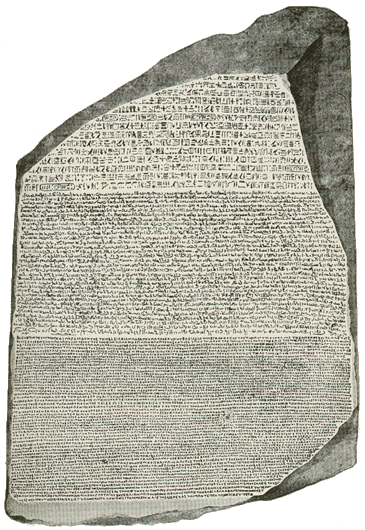
\includegraphics[width=4in]{images/RosettaStone.png}

}
% }}}


% Scientific Method: Candle 4; write something surprising you learned {{{
\pageNoBottomDiv{

The majority of writing consisted of geneologies, legal codes, and fantastic
stories. But some writing represented progress in philosophy and mathematics,
eventually culminating in the invention of the scientific method.

\divider

\blockquote{Mathematics is the gate and key of the sciences... Neglect of
mathematics works injury to all knowledge, since he who is ignorant of it
cannot know the other sciences or the things of this world. And what is worse,
men who are thus Ignorant are unable to perceive their own ignorance and so do
not seek a remedy.}{Roger Bacon, Opus Majus (1266)}

} %}}}
% Scientific method {{{
\sidePage{

\stagedir{
Using the third candle, which represents writing, light the fourth candle to
represent the scientific method.

\candelabrum{images/candelabrum4.png}

% TODO: Replace this with a better written thing
Then, everyone write down something surprising you learned in the past week,
and put it in the middle. When everyone has written something, continue to the
next page.}

\divider

}
% }}}


% Black Death: Blow out candle 4 {{{
\page{

The scientific method, combined with writing and a university system, marked
the start of an accumulation of knowledge. This could have marked the beginning
of a slow transition into the modern era. Instead, 81 years after Roger Bacon,
history was derailed by a great plague.

\divider

\stagedir{Take the fourth candle, which represents the progress of science.
Hold it, while you read the quote.}

\blockquote{The seventh year after it began, it came to England and first began
in the towns and ports joining on the seacoasts, in Dorsetshire, where, as in
other counties, it made the country quite void of inhabitants so that there
were almost none left alive. ... But at length it came to Gloucester, yea even
to Oxford and to London, and finally it spread over all England and so wasted
the people that scarce the tenth person of any sort was left alive.}{Geoffrey
the Baker, Chronicon Angliae (1360)}

\stagedir{Blow out the candle. Then return it to its place on the candelabrum.}

\candelabrum{images/candelabrum4b.png}

} %}}}
% Black Death cont'd {{{
\page{

The plague killed about half the population of Europe during a four-year
period, and it recurred repeatedly throughout the next three centuries killing
double-digit percentages of the population each time. Between plagues, wars,
and famines, there was little time to build or preserve knowledge.

} %}}}


% Printing press: Re-light candle 4 {{{
\page{

Preserving knowledge required redundancy. In 1439, during the European
Renaissance, Gutenberg perfected a device to do just that.

\divider

\blockquoteUnmarked{``Pray, friend Martin, how many impressions can be made by
this press in a day?'' ``About three hundred, if we work it constantly.'' ``Is
it possible!'' exclaimed Peter. ``Now indeed will books multiply. What will the
plodding copyists say to this?''}{Emily Clemens Pearson, Gutenberg and the Art
of Printing (1870)}

\stagedir{Take the fourth candle, which represents the progress of science.

Touch it to each of the other three candles in turn, until it is lit. Then
return it to its place on the candelabrum.}

\candelabrum{images/candelabrum4.png}

} %}}}

% Age of Progress

% Galileo 1610, Halley/Newton 1687{{{
\page{

\stagedir{Take the fourth candle, which represents science. Hold it, while you
read the quote, then pass it directly to the next person. Repeat for each quote
in this section.}

\blockquote{By the aid of a telescope any one may behold this in a manner which so
distinctly appeals to the senses that all the disputes which have tormented
philosophers through so many ages are exploded at once by the indisputable
evidence of our eyes, and we are freed from wordy disputes upon this subject,
for the Galaxy is nothing else but a mass of innumerable stars planted together
in clusters.}{Galileo, The Starry Messenger (1610)}
% Footnote: Some words have been modernized. Sidereal->Starry, irrefragable->indisputable.

\divider

\blockquote{Matters that vexed the minds of ancient seers,\newline
And for our learned doctors often led\newline
to loud and vain contention, now are seen\newline
In reason's light, the clouds of ignorance\newline
Dispelled at last by science. Those on whom\newline
Delusion cast its gloomy pall of doubt,\newline
Upborne now on the wings that genius lends,\newline
May penetrate the mansions of the gods\newline
And scale the heights of heaven. O mortal men,\newline
Arise! And, casting off your earthly cares,\newline
Learn ye the potency of heaven-born mind,\newline
Its thought and life far from the herd withdrawn!}{Edmund Halley, preface to Newton's Principia Mathematica (1687)}

} %}}}


% Bayes 1763, Watt 1765 {{{
\page{
\blockquote{By calculations similar to these may be determined universally, what
expectations are warranted by any experiments, according to the different number
of times in which they have succeeded and failed; or what should be thought of
the probability that any particular cause in nature, with which we have any
acquaintance, will or will not, in any single trial, produce an effect that has
been conjoined with it.}{Rev. Thomas Bayes, An Essay towards solving a Problem
in the Doctrine of Chances (1763)}

\divider

\blockquote{I was thinking upon the engine at the time, and had gone as far as
the herd's house, when the idea came into my mind that as steam was an elastic
body it would rush into a vacuum, and if a communication were made between the
cylinder and an exhausted vessel it would rush into it, and might be there
condensed without cooling the cylinder. I then saw that I must get rid of the
condensed steam and injection-water if I used a jet as in Newcomen's engine.
Two ways of doing this occurred to me. ... I had not walked farther than the
golf-house when the whole thing was arranged in my mind.}{James Watt (1765)}

} %}}}

% Mendeleev 1864, Bell 1876, candle 5 {{{
\page{

\blockquote{I saw in a dream a table where all elements fell into place as
required. Awakening, I immediately wrote it down on a piece of paper, only in
one place did a correction later seem necessary.}{Dmitri Mendeleev (1864)}

\divider

\blockquote{I then shouted into the mouthpiece the following sentence: Mr.
Watson, Come here, I want to see you. To my delight he came and declared that
he had heard and understood what I said. I asked him to repeat the words. He
answered, ``You said, Mr. Watson come here I want to see you.''}{Alexander Graham Bell (1876)}

\divider

\blockquote{I speak without exaggeration when I say that I have constructed
3,000 different theories in connection with the electric light, each one of
them reasonable and apparently likely to be true. Yet only in two cases did my
experiments prove the truth of my theory. My chief difficulty was in
constructing the carbon filament. ... Every quarter of the globe was ransacked
by my agents, and all sorts of the queerest materials used, until finally the
shred of bamboo, now utilized by us, was settled upon.}{Thomas Edison (1890)}

} %}}}


% The urn of inventions {{{
\page{

\stagedir{Return the candle to the candelabrum.}

Take a minute to notice the time scale of these discoveries. Each one
significantly changed society, and each change was at least mostly for the
better.

\divider

\blockquote{If we continually sample from the urn of possible technological
discoveries before implementing effective means of global coordination,
surveillance, and/or restriction of potentially hazardous information, then we
risk eventually drawing a black ball: an easy-to-make intervention that causes
extremely widespread harm and against which effective defense is
infeasible}{Nick Bostrom (2013)}

\divider

As we enter the thirties and forties, many of the rules on which human society
was built have given way to science and industry. Prior to this point,
technological progress moved at the speed of civilization, and its effects were
mainly effects on societies. Each technology has a name attached, but those
names do not matter much.

} %}}}

% Industrial era

% CUT: Industrialization {{{
%\page{
%
%With reason and learning, with lightning and steel, humans built on a scale
%never before seen. As we created tools and infrastructure, small gains in
%efficiency compounded, and compounded, and compounded again, leading to yet
%better tools and yet more infrastructure. We built tractors that feed cities,
%railroads that span continents, and economies that coordinate thousands of
%millions of humans.
%
%\blockquote{If a device would save in time just 10 per cent. or increase results 10 per
%cent., then its absence is always a 10 per cent. tax. If the time of a person
%is worth fifty cents an hour, a 10 per cent. saving is worth five cents an
%hour. ... Save ten steps a day for each of twelve thousand employees and you will
%have saved fifty miles of wasted motion and misspent energy. Those are the
%principles on which the production of my plant was built up.}{Henry Ford, ``My Life and Work'' (1922)}
%
%\divider
%
%} % }}}
% Political Science {{{
\page{
% Sneaky quote
\blockquoteUnattributed{Those material inventions, beginning with the use of stones as
weapons, which led to the domestication of animals, the production of fire by
artificial means, down to the marvellous inventions of our own days, show
clearly that an individual was the originator in each case. The nearer we come
to our own time and the more important and revolutionary the inventions become,
the more clearly do we recognize the truth of that statement. All the material
inventions which we see around us have been produced by the creative powers and
capabilities of individuals.}

\divider

Each of the inventors mentioned so far has been basically a good person,
interested in finding truth, improving society or, at worst, making a business
for themself. Newton mastered calculus; Watt mastered steam; Edison mastered
electricity. History was changed by their inventions, but not by their
characters.

But in 1939, someone figured out \emph{power} - what we would now call political
science. He learned how to effectively use film and radio for propaganda, when
these were new. And this time, it matters a great deal who he was. He was the
writer of the last quote. And he is now widely considered the most evil man
ever to have lived.

} % }}}


% World War 2 {{{
\page{

\blockquote{I should like to call attention to the fact that the principle of
parliamentarian democracy, whereby decisions are enacted through the majority
vote, has not always ruled the world. On the contrary, we find it prevalent
only during short periods of history, and those have always been periods of
decline in nations and States.}{Adolf Hitler, Mein Kampf (1926)}

%\blockquote{In those days the following happened almost always: I presented
%myself before an assembly of men who believed the opposite of what I wished to
%say and who wanted the opposite of what I believed in. Then I had to spend a
%couple of hours in persuading two or three thousand people to give up the
%opinions they had first held, in destroying the foundations of their views
%with one blow after another and finally in leading them over to take their
%stand on the grounds of our own convictions and our philosophy of life.
%
%I learned something that was important at that time, namely, to snatch from
%the hands of the enemy the weapons which he was using in his reply. I soon
%noticed that our adversaries, especially in the persons of those who led the
%discussion against us, were furnished with a definite repertoire of arguments
%out of which they took points against our claims which were being constantly
%repeated. The uniform character of this mode of procedure pointed to a
%systematic and unified training. And so we were able to recognize the
%incredible way in which the enemy's propagandists had been disciplined, and I
%am proud today that I discovered a means not only of making this propaganda
%ineffective but of beating the artificers of it at their own work. Two years
%later I was master of that art.}{Adolf Hitler, Mein Kampf (1926)}
%
%\blockquote{The art of propaganda lies in understanding the emotional ideas of
%the great masses and finding, through a psychologically correct form, the way
%to the attention and thence to the heart of the broad masses. ... There was no
%end to what could be learned from the enemy by a man who kept his eyes open,
%refused to let his perceptions be ossified, and for four and a half years
%privately turned the stormflood of enemy propaganda over in his brain.}{Adolf Hitler, Mein Kampf (1926)}

\divider

Starting in 1939 and continuing until 1945, World War 2 killed about 60 million
people. Had it gone differently, it's likely that the entire world would have
fallen under a single totalitarian regime. This would not have meant human
extinction, exactly - but it would most likely mean the loss of humanity's
potential.

And so the world's greatest minds believed they had no choice. They had to
gather in secret, and create the atomic bomb - a weapon to destroy cities, or
the whole world.

} %}}}
% Manhattan Project: Take candle 5, and drip wax. {{{
\page{

\blockquote{Despite the vision and farseeing wisdom of our wartime heads of state, the
physicists have felt the peculiarly intimate responsibility for suggesting, for
supporting, and in the end, in large measure, for achieving the realization of
atomic weapons. Nor can we forget that these weapons as they were in fact used
dramatized so mercilessly the inhumanity and evil of modern war. In some sort
of crude sense which no vulgarity, no humor, no overstatement can quite
extinguish, the physicists have known sin; and this is a knowledge which they
cannot lose.}{Robert J. Oppenheimer (1947)}

%\stagedir{Take the fourth candle, which represents science. Hold it over the
%stack of papers until three drops of wax fall. Then use it to light the fifth
%candle, which represents industrialization.}
\stagedir{Using the fourth candle, which represents science, light the fifth
candle to represent industrialization.}

\candelabrum{images/candelabrum5.png}

} % }}}


% Postwar Progress {{{
\page{

After the war, things settled down - but the pace of progress continued.

In 1951, the first transistor.\newline
In 1952, the first hydrogen bomb.\newline
In 1953, the discovery of DNA's structure.\newline
In 1954, the first solar cell, model rocket, and nuclear submarine.\newline
In 1955, the Polio vaccine.\newline
In 1956, the first commercial nuclear power station.\newline
In 1957, Sputnik, the first orbital space flight.\newline
In 1958, the first integrated circuit.\newline
In 1959, Lunik 2, the first satellite to reach the moon.

\divider

As our technology took off - figuratively and literally - no one knew what we
would find. Predicting the future was left mostly to science fiction writers,
and their predictions were not especially accurate. But some scientists did
take important questions seriously. For example, would there be life in space?
The SETI project began in 1961, at the National Radio Astronomy Observatory in
West Virginia.

} % }}}
% Great Filter, Robin Hanson {{{
\page{

\blockquote{I wrote down all the things you needed to know to predict how hard it's going
to be to detect extraterrestrial life. And looking at them it became pretty
evident that if you multiplied all these together, you got a number, N, which
is the number of detectable civilizations in our galaxy.}{Frank Drake}

\divider

\blockquote{Humanity seems to have a bright future, i.e., a non-trivial chance
of expanding to fill the universe with lasting life. But the fact that space
near us seems dead now tells us that any given piece of dead matter faces an
astronomically low chance of begetting such a future. There thus exists a great
filter between death and expanding lasting life, and humanity faces the ominous
question: how far along this filter are we?}{Robin Hanson (1998)}

%\divider
%
%The absence of observed alien life, taken together with our current best
%estimates of how unlikely it was for life to arise and to advance to the point
%where we are now, means that there must be some filter further in our future,
%which prevents most life from spreading through the stars. Therefore, either
%our model of the past or of the universe is very substantially wrong, or there
%is an obstacle in our future which most intelligent civilizations fail to pass.
%We have several ideas about what that obstacle might be.

} % }}}


% CUT: Dartmouth Conference 1956 {{{
%\page{
%
%One thing we did \textit{not} invent in the fifties, was artificial
%intelligence. But not entirely for lack of trying. Two years before the first
%integrated circuit and 15 years before the first microprocessor, John McCarthy
%organized the Dartmouth conference to study the problem of artificial
%intelligence.
%
%\divider
%
%\blockquote{We propose that a 2 month, 10 man study of artificial intelligence
%be carried out during the summer of 1956 at Dartmouth College in Hanover, New
%Hampshire.  The study is to proceed on the basis of the conjecture that every
%aspect of learning or any other feature of intelligence can in principle be so
%precisely described that a machine can be made to simulate it. An attempt will
%be made to find how to make machines use language, form abstractions and
%concepts, solve kinds of problems now reserved for humans, and improve
%themselves. We think that a significant advance can be made in one or more of
%these problems if a carefully selected group of scientists work on it together
%for a summer.}{McCarthy et al, 1956}
%
%} % }}}
% CUT: SETI 1961, Drake equation {{{
%\page{
%
%In 1961, the Search for Extraterrestrial Intelligence (SETI) held its first
%conference at the National Radio Astronomy Observatory in West Virginia, to
%discuss what is now called the Drake Equation:
%
%In forty-odd years of searching, we have found no extraterrestrial life. Our
%best estimates for the Drake equation, however, suggest that there should be.
%This is the Fermi Paradox: where is everybody?
%
%} % }}}


% Cuban Missile Crisis 1962: Drip wax {{{
\page{
In 1962, the cold war between the United States and the Soviet Union reached a
crisis. US destroyers under orders to enforce a naval quarantine off Cuba did
not know that the submarines the Soviets had sent to protect their ships were
carrying nuclear weapons. So the Americans began firing depth charges to force
the submarines to the surface, a move the Soviets on board interpreted as the
start of World War III.

\divider

\blockquote{We're going to blast them now! We will die, but we will sink them
all. We will not  disgrace our navy,}{Captain Valentin Grigorievitch Savitsky (1962)}

\stagedir{Take the fifth candle, which represents industry. Hold it over
the stack of papers until three drops of wax fall.}

} % }}}
% Arkhipov {{{
\page {
The launch of the submarine's nuclear torpedo required the consent of all three
senior officers aboard: Captain Valentin Grigorievitch Savitsky, political
officer Ivan Semonovich, and second in command Vasili Arkhipov.

Arkhipov was alone in refusing to launch the nuke, insisting the submarine
surface to receive orders from Moscow. Had he chosen differently, the likely
result would have been all-out nuclear war.

\begin{center}
	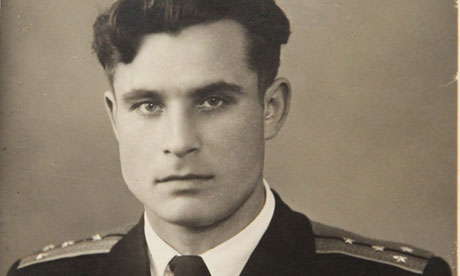
\includegraphics[width=3.0in]{images/VasiliArkhipov.jpg}
\end{center}

} % }}}


% 1963: IJ Good, Superintelligence: Place an unlit candle in the last spot {{{
\page{

Meanwhile, technology marched on. And for the first time, it seemed that
technological progress might not go on forever, but build towards an ultimate
conclusion.

\divider

\blockquote{Let an ultraintelligent machine be defined as a machine that can far surpass
all the intellectual activities of any man however clever. Since the design of
machines is one of these intellectual activities, an ultra-intelligent machine
could design even better machines; there would then unquestionably be an
``intelligence explosion,'' and the intelligence of man would be left far behind.
Thus the first ultraintelligent machine is the last invention that man need
ever make, provided that the machine is docile enough to tell us how to keep it
under control.}{I.J. Good, Speculations Concerning the First Ultraintelligent Machine (1963)}

\stagedir{Place an unlit candle in the last spot, to represent future
technology.}

\candelabrum{images/candelabrum5b.png}

} % }}}
% Moore's Law 1965: Light candle 6, Computers {{{
\page{

Two years later, Gordon Moore famously observed:

\blockquote{The complexity for minimum component costs has increased at a rate
of roughly a factor of two per year. Certainly over the short term this rate
can be expected to continue, if not to increase. Over the longer term, the rate
of increase is a bit more uncertain, although there is no reason to believe it
will not remain nearly constant for at least 10 years. That means by 1975, the
number of components per integrated circuit for minimum cost will be 65,000.}{Gordon Moore (1965)}

\vspace*{1.2in}

\stagedir{Using the fifth candle, which represents industrialization, light the
sixth candle to represent the invention of computers.}

\candelabrum{images/candelabrum6.png}

%\divider
%
%Moore's Law has been rephrased many times, to talk about slightly different
%things - clock rate, computation speed, cost per computation speed, cost per
%computation. Some of these phrasings must eventually face fundamental physical
%limits - but some of them need not. For now, the speed of computation is
%increasing at the slightly slower rate of roughly a factor of two every other
%year. It shows no sign of stopping.

} % }}}


% Moore's Law of Mad Science; Moon landing {{{
\page {

\blockquote{Moore's Law of Mad Science: Every 18 months, the IQ required to
destroy the world drops by 1 point.}{Source unknown (2005)}

\divider

Meanwhile, the rockets that had first been developed for war were turned to
exploration as well:

\blockquote{Here men from the planet Earth first set foot upon the Moon July
1969, A.D.  We came in peace for all mankind}{Apollo 11 Plaque (1969)}

} % }}}
% CUT: AI Winter {{{
%\page{
%
%Compared to landing on the moon, computers were just not that impressive. In
%1973 the British Science Research Council commissioned James Lighthill to
%evaluate the state of artificial intelligence:
%
%\blockquote{Most workers in AI research and in related fields confess to a
%pronounced feeling of disappointment in what has been achieved in the past
%twenty-five years. Workers entered the field around 1950, and even around 1960,
%with high hopes that are very far from having been realized in 1972. In no part
%of the field have the discoveries made so far produced the major impact that
%was then promised.}{James Lighthill (1973)}
%
%\divider
%
%So began the AI winter: a period of pessimism, reduced funding, and minimal
%progress. We now know that AI is hard; how hard exactly, we don't know. Since
%then, Moore's Law has continued - and so, every year, the difficulty drops a
%little bit.
%
%} % }}}
% Population growth {{{
\page{

Lest we forget how difficult predicting the future is, here is one predicted
disaster that did not come to pass.

\divider

\blockquote{The battle to feed all of humanity is over. In the 1970s and 1980s
hundreds of millions of people will starve to death in spite of any crash
programs embarked upon now. At this late date nothing can prevent a substantial
increase in the world death rate, although many lives could be saved through
dramatic programs to "stretch" the carrying capacity of the earth by increasing
food production and providing for more equitable distribution of whatever food
is available. But these programs will only provide a stay of execution unless
they are accompanied by determined and successful efforts to at population
control. Population control is the conscious regulation of the numbers of human
beings to meet the needs not just of individual families, but of society as a
whole.
\newline\newline
Nothing could be more misleading to our children than our present affluent
society. They will inherit a totally different world, a world in which the
standards, politics and economics of the past decade are dead. As the most
influential nation in the world today, and its largest consumer, the United
States cannot stand isolated. We are today involved in the events leading to
famine and ecocatastrophe; tomorrow we may be destroyed by them.}{Paul Ehrlich (1968)}

} %}}}


% CUT: Flynn Effect {{{
%\page{
%At this point, it's worth noting another effect, something like Moore's Law,
%which also continues year after year: the Flynn effect. Ever since mental tests
%were introduced, the mean IQ of Americans has been rising at a rate of about .3
%points per year. I went to James Flynn's paper on this, published in 1984,
%expecting to find a discussion of advancing intelligence, pick out an
%illustrative quote and move on. That is not what I found.
%
%While technology changes rapidly, it is often said that human nature doesn't
%change. Rising IQs are a change to human nature, but a comprehensible one; it
%is mostly a matter of the average people becoming more like the best people.
%But human nature changes in more ways than one, and while Flynn was interested
%in rising IQ test results, his goal was to reconcile them with falling scores
%on a different test, the Scholastic Aptitude Test or SAT.
%
%\divider
%
%\blockquote{Our analysis dictates the conclusion that American 18-year-olds have
%deteriorated .48 to .96 SDU in terms of a total package consisting of
%motivation, study habits, self-discipline, and acquired verbal and writing
%skills. Which is to say that only the upper, 17\% to 32\% of today's 18-year-olds
%can match the upper half of young people as recently as 1963! The calculations
%above should not be taken literally of course: They are merely meant to show
%that if both IQ gains and SAT losses are taken to be real, rather than
%artifacts of sampling error, then the deterioration of non-IQ personal traits
%among young Americans must have been very great.}{James R. Flynn (1984)}
%
%\divider
%
%I don't know how to compare the personality traits of populations over time,
%but I do know this: the world is suddenly filled with stressors and drugs and
%superstimuli that enable humans to go insane in a variety of novel and exciting
%ways, and we keep inventing new ones. Sometimes, humans go insane in ways that
%are dangerous to those around them, and sometimes they go insane from positions
%of power.
%
%} % }}}

% Petrov incident - drip wax {{{
\pageNoBottomDiv{
Moving away from the long-term trends and back to concrete events, we now reach
the historical event that is today's namesake: the Petrov incident. On
September 26, 1983, Stanislav Petrov was the duty officer at the Oko nuclear
early warning system.

\divider

\blockquote{An alarm at the command and control post went off with red lights blinking on
the terminal. It was a nasty shock. Everyone jumped from their seats, looking
at me. What could I do? There was an operations procedure that I had written
myself. We did what we had to do. We checked the operation of all systems - on
30 levels, one after another. Reports kept coming in:  All is correct; the
probability factor is two. ... The highest.}{Stanislav Petrov}

%\stagedir{Take the fifth candle, which represents industry. Hold it over
%the stack of papers until three drops of wax fall.}

\divider

\begin{center}
	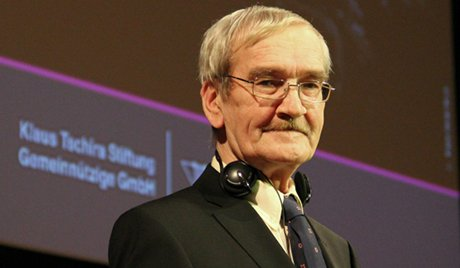
\includegraphics[width=3.0in]{images/StanislavPetrov.jpg}
\end{center}

} % }}}
% Petrov incident {{{
\page{
\blockquote{I imagined if I'd assume the responsibility for unleashing the third World War
- and I said, no, I wouldn't. ... I always thought of it. Whenever I came on
duty, I always refreshed it in my memory.}{Stanislav Petrov}

\divider

Had he followed procedure, and reported up the chain of command that the
Americans had launched missiles, this could have set off a nuclear war. So
instead of telling his superiors what the system was saying, Petrov told his
superiors that it was a false alarm - despite not really knowing this was the
case.

\divider

%\blockquoteUnattributed{You can't possibly analyze things properly within a
%couple of minutes ... All you can rely on is your intuition. I had two
%arguments to fall back on. First, missile attacks do not start from just one
%base. Second, the computer is, by definition, brainless. There are lots of
%things it can mistake for a missile launch.}

At the time, he received no award. The incident embarrassed his superiors and
the scientists responsible for the system, so if he had been rewarded, they
would have to be punished. (He received the International Peace Price thirty
years later, in 2013).

Things eventually calmed down. The Soviet Union dissolved. Safeguards were put
on most of the bombs, to prevent the risk of accidental (or deliberate but
unauthorized) detonation. 

} %}}}

%%%%%%%%%%%%%%%%%%%%%%%%%%%%%%%%%%%%%%%%%%%%%%%%%%%%%%%%%%%%%%%%%%%%%%%%%%%%%%%

% Ozone layer {{{
\page{
In 1985, Joe Farman, Brian Gardiner, and Jonathan Shanklin made a disturbing
discovery. The ozone layer, the part of our atmosphere that filters out most UV
radiation, was disappearing due to chlorofluorocarbon pollution. Just two years
later a treaty was written to ban the use of CFCs, and two years after that, in
1989, it was in effect. As of today, every country in the United Nations has
ratified the Montreal protocol.

\divider

\blockquote{The hole in the ozone layer is a kind of skywriting. At first it
seemed to spell out our continuing complacency before a witch's brew of deadly
perils. But perhaps it really tells of a newfound talent to work together to
protect the global environment.}{Carl Sagan (1998)}

} % }}}

% AI risk {{{
\page{

But not every threat to humanity is as easy to understand or address as
nuclear weapons or the ozone layer.

\divider

\blockquote{An unFriendly AI with molecular nanotechnology (or other rapid
infrastructure) need not bother with marching robot armies or blackmail or
subtle economic coercion. The unFriendly AI has the ability to repattern all
matter in the solar system according to its optimization target. This is fatal
for us if the AI does not choose specifically according to the criterion of how
this transformation affects existing patterns such as biology and people. The
AI does not hate you, nor does it love you, but you are made out of atoms which
it can use for something else. The AI runs on a different timescale than you
do; by the time your neurons finish thinking the words ``I should do something''
you have already lost}{Eliezer Yudkowsky, Artificial Intelligence as a Positive
and Negative Factor in Global Risk (2006)}

%\divider
%
%At the Global Catastrophic Risk Conference in Oxford (17-20 July, 2008) an
%informal survey was circulated among participants, asking them to make their
%best guess at the chance that there will be disasters of different types before
%2100. The median estimate was a 19\% chance of human extinction.

} % }}}
% Differential Technological Advancement, AI Progress {{{
\page{

\blockquote{What we do have the power to affect (to what extent depends on how
we define ``we'') is the rate of development of various technologies and
potentially the sequence in which feasible technologies are developed and
implemented. Our focus should be on what I want to call differential
technological development: trying to retard the implementation of dangerous
technologies and accelerate implementation of beneficial technologies,
especially those that ameliorate the hazards posed by other
technologies.}{Nick Bostrom (2002)}

\stagedir{Place an unlit candle in the second-to-last spot, to represent
alternate possible futures.}

\candelabrum{images/candelabrum6b.png}

} %}}}

% AI risk continued {{{
% TODO: This page is weak
\page{

\blockquote{Though I would have liked my chances in a rematch in 1998 if I were
better prepared, it was clear then that computer superiority over humans in
chess had always been just a matter of time.}{Garry Kasparov, world Chess
champion, after losing to IBM's Deep Blue}

\divider

Twenty-four years after the Lighthill Report declared AI a failure, in 1997 the
computer program Deep Blue defeated World Chess Champion Garry Kasparov. Chess,
it turns out, was not as difficult as we thought. Fully general intelligence,
however, remained out of reach.

\divider

\blockquote{I, for one, welcome our new computer overlords.}{Ken Jennings,
Jeopardy champion, after losing to IBM's Watson}

\divider

Jeopardy, it turns out, was not as difficult as we thought. But fully general
intelligence remains out of reach.

We think that it is difficult.

} %}}}
% AI risk 3 {{{
% TODO: Rewrite this page
\page{

Can progress in computing truly threaten us? So far, as science and technology
have advanced, human flourishing has advanced in tandem. We have built horrors,
to be sure: machine guns and mustard gas and even nuclear bombs. But their
aggregate impact on human life pales in comparison to that of aviation and
telecommunications and antibiotics and ten thousand other miracles.

Perhaps artificial intelligence will be made safe too, but the example of
nuclear weapons shows that this is not certain. But for the actions of Arkhipov
and Petrov, we could have wiped out not just ourselves, but our children's
children, and the possibility of ever reaching beyond the Earth. 

Which brings us to our next crisis, in 2012, and this one is not so clear.

} % }}}

% A/H5N1 NSABB report {{{
\page{
\blockquote{Recently, several scientific research teams have achieved some success in
modifying influenza A/H5N1 viruses such that they are now transmitted
efficiently between mammals, in one instance with maintenance of high
pathogenicity. ... The NSABB was unanimous that communication of the results in
the two manuscripts it reviewed should be greatly limited in terms of the
experimental details and results. The life sciences have reached a cross-roads.
The direction we choose and the process by which we arrive at this decision
must be undertaken as a community and not relegated to small segments of
government, the scientific community or society. Physicists faced a similar
situation in the 1940s with nuclear weapons research, and it is inevitable
that other scientific disciplines will also do so.}{Natl. Security Advisory
Board for Biosecurity, (2012)}

\divider

After several months, the decision was reversed, and a revised version of the
bird flu paper was approved for publication, by a vote of 12 to 6.

\divider

And now we're at the present day. So far, humanity has neither destroyed
itself, nor reached a safe position. But this is only the middle of the story.
We approach the climax of human history, where we will either destroy ourselves,
or spread through the stars.

} %}}}

% CUT: Differential intellectual progress 2 {{{
%\page{
%
%\blockquote{Differential intellectual progress consists in prioritizing risk-reducing
%intellectual progress over risk-increasing intellectual progress. As applied to
%AI risks in particular, a plan of differential intellectual progress would
%recommend that our progress on the scientific, philosophical, and technological
%problems of AI safety outpace our progress on the problems of AI capability
%such that we develop safe superhuman AIs before we develop (arbitrary)
%superhuman AIs. Our first superhuman AI must be a safe superhuman AI, for we
%may not get a second chance. With AI as with other technologies, we may become
%victims of ``the tendency of technological advance to outpace the social control
%of technology''.}{Luke Muehlhauser, Anna Salamon (2012)}
%
%\stagedir{Place an unlit candle in the eighth spot, to represent safe artificial intelligence.}
%
%}
% }}}

%%%%%%%%%%%%%%%%%%%%%%%%%%%%%%%%%%%%%%%%%%%%%%%%%%%%%%%%%%%%%%%%%%%%%%%%%%%%%%%

% Ending

% By the power of these candles... {{{
\page{

\stagedir{Take the first candle. Read the following, then return it.}
\blockspacing{By the power of fire, I am animated, freed from the demands of mere subsistence, and able to care about the future.}

\divider

\stagedir{Take the second candle. Read the following, then return it.}
\blockspacing{By the power of language, I am able to share what I know of the world and of the future, and to hear what others have learned before me.}

\divider

\stagedir{Take the third candle. Read the following, then return it.}
\blockspacing{By the power of writing, my words echo through time and space. I take part in a dialogue of billions, and together we choose the future we want.}

} %}}}
% By the power of these candles... {{{
\page{

\stagedir{Take the fourth candle. Read the following, then return it.}
\blockspacing{By the power of science, I know the true nature of the world I live in. I live in a world that obeys physical laws, which govern the outcomes of my actions, and so I can know the consequences of what I do.}

\divider

\stagedir{Take the fifth candle. Read the following, then return it.}
\blockspacing{By the power of industry, the world I live in is transformed. I can transform it further, if I choose.}

\divider

\stagedir{Take the sixth candle, and read the following.}
\blockspacing{By the power of computation, the power of my mind is amplified. I can see whole the knowledge of mankind, a great fractal pattern of summaries and details and summaries-of-summaries and details-of-details and search it all with a word.}
\stagedir{Take the candle and hold it near the seventh and eight candles, which represent good and bad futures. Then pull it back, and return it to its place.}

} %}}}

% We choose... {{{
\page{

\stagedir{Read the following together.}

We, as individuals, must each choose:\newline
Will we stand aside, as history continues?\newline
Will we be heroes, moving to the center of the action?\newline
Will we find the heroes and be their allies, up close or from afar?\newline
It's easy to imagine ourselves as powerless, and take that as an excuse.\newline
\newline
Let us not forget what power we have, and what we truly are.

} %}}}

\pagenumbering{gobble}
\sidePage{}

% Rear cover {{{
\sidePage{
}
% }}}

\end{document}
